\section{Cuantiles}
Como consecuencia del estudio de la mediana, surgen otros estadígrafos que dividen a las observaciones en otras proporciones y no solo en mitades como lo hace la media, los estadígrafos mas frecuentes de este tipo en el análisis estadístico son:
\begin{itemize}
\item \textbf{Cuartiles $(Q_i)$}
\item \textbf{Deciles $(D_i)$}
\item \textbf{Percentiles $(P_i)$}
\end{itemize}
Los cuantiles se emplean para describir el comportamiento de una población y sus resultados se expresan en tanto por ciento.
\subsection{Cuartiles $(Q_i)$}
Son valores que dividen a un conjunto de datos ordenados de forma ascendente o descendente en cuatro partes iguales:
\begin{center}
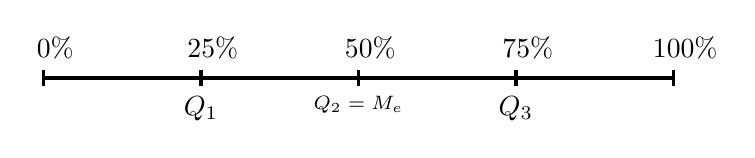
\begin{tikzpicture}
\draw[very thick] (0,0) -- + (8,0);
\foreach \i/\j [count=\x from 0] in {0/ , 25/$Q_1$, 50/{\scriptsize $Q_2=M_e$},   75/$Q_3$, 100/ }
\draw[very thick] (2*\x,0.1) node[above,xshift=1ex] {\i\%} -- + (0,-0.2) node[below] {\j};
\end{tikzpicture}
\end{center}
\subsection{Deciles $(D_i)$}
Son valores que dividen a un conjunto de datos ordenados de forma ascendente o descendente en diez partes iguales:
\begin{center}
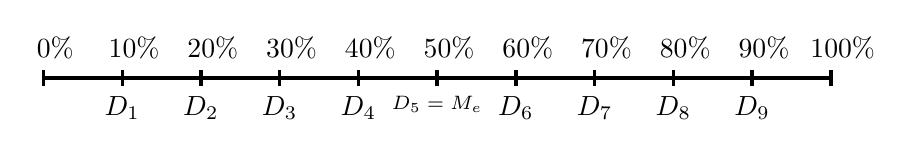
\begin{tikzpicture}
\draw[very thick] (0,0) -- + (10,0);
\foreach \i/\j [count=\x from 0] in {0/ , 10/$D_1$, 20/$D_2$, 30/$D_3$, 40/$D_4$,50/{\scriptsize $D_5=M_e$},60/$D_6$,70/$D_7$,80/$D_8$,90/$D_9$,100/ }
\draw[very thick] (\x,0.1) node[above,xshift=1ex] {\i\%} -- + (0,-0.2) node[below] {\j};
\end{tikzpicture}
\end{center}
\subsection{Percentiles $(P_i)$}
Son valores que dividen a un conjunto de datos ordenados de forma ascendente o descendente en cien partes iguales:
\begin{center}
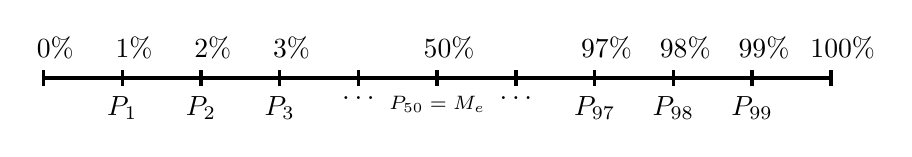
\begin{tikzpicture}
\draw[very thick] (0,0) -- + (10,0);
\foreach \i/\j [count=\x from 0] in {0/ , 1/$P_1$,2/$P_2$,{3}/$P_3$}
\draw[very thick] (\x,0.1) node[above,xshift=1ex] {\i\%} -- + (0,-0.2) node[below] {\j};
\foreach \i/\j [count=\x from 4] in {/$\ldots$,50{$\%$}/{\scriptsize $P_{50}=M_e$},/$\ldots$}
\draw[very thick] (\x,0.1) node[above,xshift=1ex] {\i} -- + (0,-0.2) node[below] {\j};

\foreach \i/\j [count=\x from 7] in {97/$P_{97}$ , 98/$P_{98}$,99/$P_{99}$,{100}/}
\draw[very thick] (\x,0.1) node[above,xshift=1ex] {\i\%} -- + (0,-0.2) node[below] {\j};

\end{tikzpicture}
\end{center}
\subsection{Cálculo de Cuantiles}
\subsubsection{Para datos Originales}
\begin{itemize}
\item \textbf{Cuartiles:}
$$Q_i=x_{\frac{i(n+1)}{4}}$$
\item \textbf{Deciles:}
$$D_i=x_{\frac{i(n+1)}{10}}$$
\item \textbf{Percentiles:}
$$P_i=x_{\frac{i(n+1)}{100}}$$
\end{itemize}
\subsubsection{Para datos Agrupados}
\begin{itemize}
\item \textbf{Cuartiles:}
$$Q_i=y_{j-1}'+C_j\dfrac{i\frac{n}{4}-F_{j-1}}{f_j}$$
\item \textbf{Deciles:}
$$D_i=y_{j-1}'+C_j\dfrac{i\frac{n}{10}-F_{j-1}}{f_j}$$
\item \textbf{Percentiles:}
$$P_i=y_{j-1}'+C_j\dfrac{i\frac{n}{100}-F_{j-1}}{f_j}$$
\end{itemize}
\subsection{Ejemplos}